% Provenance (never printed): cycle 3 "La planete Terre" and geography
% (weather and climate; reading a climate chart; the great climate zones of
% the world, hot, temperate and cold); see sources/book1/PROVENANCE.md.
% Book 1, grade 5, chapter 2.
\chapter{الطقس والمناخ}\label{ch:g5:weather-and-climate}

في الأسبوع الثاني من يناير، تصل إلى المدرسة بطاقتان بريديتان. الأولى، من
ابنة عم لينا، تُظهر أطفالًا يبنون قصرًا من \omterm{def:g3:stones-pebbles-sand:sand}{الرمل} على شاطئ مشمس تحت أشجار
النخيل. والثانية، من جدة توم، تُظهر أطفالًا يبنون رجل \omterm{def:g4:clouds-rain-snow:precipitation}{ثلج} في حديقة مكسوة
\omterm{def:g4:clouds-rain-snow:precipitation}{بالثلج}. يسأل توم: «كيف يكون صيف وشتاء في الأسبوع
نفسه؟»

ليس \omterm{def:g1:watching-the-weather:weather}{طقس} يوم واحد هو ما يختلف كل هذا الاختلاف بين المكانين. بل \omterm{def:g1:watching-the-weather:weather}{الطقس} الذي
يعرفانه، سنة بعد سنة: أي مناخهما.

\begin{omfigure}
\begin{minipage}[b]{0.48\linewidth}\centering

\includegraphics[width=\linewidth]{images/book1/ai/g5-beach-postcard.jpg}
\end{minipage}\hfill
\begin{minipage}[b]{0.48\linewidth}\centering

\includegraphics[width=\linewidth]{images/book1/ai/g5-snowman-postcard.jpg}
\end{minipage}

{\small بطاقتان بريديتان من الأسبوع نفسه من يناير: شاطئ مشمس وحديقة
مكسوة \omterm{def:g4:clouds-rain-snow:precipitation}{بالثلج}.}
\end{omfigure}

\begin{recall}
\omterm{def:g1:watching-the-weather:weather}{الطقس} هو حال الهواء في مكان ولحظة معيّنين: مشمس، غائم، ماطر، مثلج، عاصف
(\cref{ch:g1:watching-the-weather}). ومقياس الحرارة يقيس درجة حرارة الهواء،
بالدرجات المئوية؛ \omterm{def:g4:clouds-rain-snow:rain-gauge}{ومقياس المطر} يقيس \omterm{def:g4:clouds-rain-snow:precipitation}{المطر}، بالمليمترات
(\cref{ch:g4:clouds-rain-snow}). \omterm{def:g3:continents-and-oceans:equator}{وخط الاستواء} يدور حول وسط \omterm{def:g3:continents-and-oceans:globe}{مجسم الكرة
الأرضية}، في منتصف المسافة بين \omterm{def:g3:continents-and-oceans:poles}{القطب الشمالي} \omterm{def:g3:continents-and-oceans:poles}{والقطب الجنوبي}
(\cref{ch:g3:continents-and-oceans}). وقد بيّنت كتب الفيزياء أن الأرض تدور
حول الشمس في سنة واحدة، وأن فصولها تأتي من ميل محورها: ففي الصيف تصعد الشمس
أعلى في السماء وتطول
الأيام.
\end{recall}

\section{الطقس هو اليوم، والمناخ هو المعتاد}

يتغير \omterm{def:g1:watching-the-weather:weather}{الطقس} من يوم إلى يوم، بل من ساعة إلى ساعة. أما \omterm{def:g5:weather-and-climate:climate}{المناخ} فشيء
آخر.

\begin{definition}[المناخ]\label{def:g5:weather-and-climate:climate}
\emph{المناخ}\index{مناخ} لمكان ما هو \omterm{def:g1:watching-the-weather:weather}{الطقس} الذي يعرفه عادة، شهرًا بعد شهر،
على مدى سنين كثيرة: كم يكون كل فصل دافئًا أو باردًا، رطبًا أو جافًا. ويحسبه
علماء \omterm{def:g1:watching-the-weather:weather}{الطقس} بأخذ متوسط قياسات
30 سنة.
% ledger: wmo:normal-30yr
\end{definition}

«إنها تمطر هذا الصباح» جملة عن \omterm{def:g1:watching-the-weather:weather}{الطقس}. «إنها تمطر كثيرًا في الخريف هنا» جملة
عن \omterm{def:g5:weather-and-climate:climate}{المناخ}. ويوم بارد واحد في الصيف لا يغيّر \omterm{def:g5:weather-and-climate:climate}{المناخ}؛ إنه مجرد \omterm{def:g1:watching-the-weather:weather}{طقس} غير
معتاد.

علماء \omterm{def:g1:watching-the-weather:weather}{الطقس} في العالم كله يتبعون القاعدة نفسها: يأخذون متوسط
30 سنة من القياسات. والمتوسطات المستعملة اليوم هي متوسطات السنوات
من 1991 إلى 2020.
% ledger: wmo:normal-30yr

\section{المخطط المناخي}

لنبين \omterm{def:g5:weather-and-climate:climate}{مناخ} مكان في صورة واحدة، نرسم مخططًا.

\begin{definition}[المخطط المناخي]\label{def:g5:weather-and-climate:climate-chart}
\emph{المخطط المناخي}\index{مخطط مناخي} يبين، لكل شهر من أشهر السنة، متوسط
درجة الحرارة في مكان ما (منحنى) ومتوسط كمية \omterm{def:g4:clouds-rain-snow:precipitation}{المطر} \omterm{def:g4:clouds-rain-snow:precipitation}{والثلج} التي تسقط فيه
(أعمدة، بالمليمترات من الماء).
\end{definition}

\begin{omfigure}
\begin{tikzpicture}
  \begin{axis}[name=pax, width=0.55\linewidth, height=5.6cm, ymin=0, ymax=400,
      axis y line*=right, axis x line=none, ybar, bar width=7pt,
      ytick={0,100,...,400}, ylabel={\foreignlanguage{arabic}{المطر \babelsublr{(mm)}}}, xmin=0.4, xmax=12.6,
      tick label style={font=\scriptsize}, label style={font=\scriptsize},
      ylabel style={blue!60!black}]
    \addplot[fill=blue!40, draw=blue!60!black]
      table[x=month, y=prcp_mm] {figdata/out/grade-5-climate_charts-seattle.dat};
  \end{axis}
  \begin{axis}[width=0.55\linewidth, height=5.6cm, ymin=-30, ymax=40,
      axis y line*=left, axis x line*=bottom, xmin=0.4, xmax=12.6,
      xtick={1,...,12}, xticklabels={1,2,3,4,5,6,7,8,9,10,11,12},
      ytick={-30,-20,...,40}, ylabel={\foreignlanguage{arabic}{درجة الحرارة \babelsublr{($^\circ$C)}}},
      tick label style={font=\scriptsize}, label style={font=\scriptsize},
      ylabel style={red!70!black}]
    \addplot[red!70!black, thick, mark=*, mark size=1.3pt]
      table[x=month, y=tavg_C] {figdata/out/grade-5-climate_charts-seattle.dat};
    \draw[gray!60] (axis cs:0.4,0) -- (axis cs:12.6,0);
    \begin{scope}[every node/.style={circle, draw, fill=white, inner sep=0.8pt,
        font=\scriptsize\bfseries}]
      \node[text=red!70!black, draw=red!70!black] at (axis cs:5.5,27) {1};
      \node[text=blue!60!black, draw=blue!60!black] at (axis cs:7,-19) {2};
    \end{scope}
  \end{axis}
  \node[anchor=north west, font=\scriptsize, align=left, text width=4.2cm]
    at ($(pax.outer north east)+(0.3,-0.1)$) {%
    \textcolor{red!70!black}{\textbf{1} المنحنى الأحمر: متوسط درجة الحرارة
    في كل شهر، يُقرأ على التدريج الأيسر.}\par\smallskip
    \textcolor{blue!60!black}{\textbf{2} الأعمدة الزرقاء: متوسط المطر في كل
    شهر، يُقرأ على التدريج الأيمن.}\par\smallskip
    \textbf{3} الأعداد تحت المخطط: الأشهر، من يناير (1) إلى
    ديسمبر (12).};
\end{tikzpicture}

{\small \omterm{def:g5:weather-and-climate:climate-chart}{المخطط المناخي} لسياتل، وهي مدينة على \omterm{def:g1:landscapes-around-us:water}{الساحل} الغربي للولايات المتحدة.
متوسطات السنوات من 1991 إلى 2020 (البيانات: NOAA).}
% ledger: data:b1-noaa-normals
\end{omfigure}

\begin{method}[قراءة مخطط مناخي]\label{met:g5:weather-and-climate:reading}
\begin{enumerate}
  \item جد أدفأ شهر وأبرد شهر على المنحنى الأحمر، واقرأ درجتي حرارتهما
        على التدريج الأيسر. هل المنحنى مستوٍ (درجة الحرارة نفسها طوال
        السنة) أم يرتفع وينخفض (فصول دافئة وفصول باردة)؟ وهل ينزل تحت
        \babelsublr{0~$^\circ$C} (الصقيع)؟
  \item جد أكثر الأشهر مطرًا وأقلها مطرًا بين الأعمدة الزرقاء، واقرأها
        على التدريج الأيمن. هل الأعمدة طويلة أم قصيرة؟ وهل هناك فصل
        جاف؟
  \item اجمع ذلك في جملة واحدة: «حار وجاف طوال السنة»، «معتدل
        ورطب، مع صيف جاف»{\ldots}
\end{enumerate}
\end{method}

\begin{example}[سياتل]\label{ex:g5:weather-and-climate:seattle}
في سياتل، أدفأ الأشهر أغسطس (نحو \babelsublr{20~$^\circ$C})، وأبردها ديسمبر
(نحو \babelsublr{6~$^\circ$C}): فالمنحنى يرتفع وينخفض، لكنه لا ينزل أبدًا تحت درجة
التجمد. وأطول الأعمدة عمود نوفمبر (نحو 160~mm)، وأقصرها عمود يوليو
(نحو 15~mm). وفي جملة واحدة: شتاء معتدل، وصيف لطيف، \omterm{def:g4:clouds-rain-snow:precipitation}{ومطر} في الخريف والشتاء،
وجفاف نسبي في الصيف. وفي السنة كلها يسقط نحو 1\,000~مليمتر من \omterm{def:g4:clouds-rain-snow:precipitation}{المطر}: أي
متر من الماء.
% ledger: data:b1-noaa-normals
\end{example}

\section{أربعة مناخات}

هذه \omterm{def:g5:weather-and-climate:climate-chart}{المخططات المناخية} لأربع مدن في الولايات المتحدة، متباعدة بعضها
عن بعض: فينيكس، في \omterm{def:g5:weather-and-climate:desert}{صحراء} أريزونا؛ وهيلو، في جزيرة هاواي وسط \omterm{def:g2:water-on-earth:ocean}{المحيط}
الهادئ؛ وسياتل، على \omterm{def:g1:landscapes-around-us:water}{الساحل} الغربي؛ وأوتكياغفيك، في أقصى شمال ألاسكا، على
\omterm{def:g1:landscapes-around-us:water}{ساحل} \omterm{def:g2:water-on-earth:ocean}{المحيط} المتجمد الشمالي.
والمخططات الأربعة تستعمل التدريجات نفسها، فنستطيع أن نقارنها بنظرة واحدة.

\begin{omfigure}
\def\gfivechart#1#2{%
\begin{tikzpicture}
  \begin{axis}[width=0.5\linewidth, height=4.6cm, ymin=0, ymax=400,
      axis y line*=right, axis x line=none, ybar, bar width=4pt,
      ytick={0,100,...,400}, xmin=0.4, xmax=12.6,
      tick label style={font=\tiny}]
    \addplot[fill=blue!40, draw=blue!60!black]
      table[x=month, y=prcp_mm] {figdata/out/grade-5-climate_charts-#1.dat};
  \end{axis}
  \begin{axis}[width=0.5\linewidth, height=4.6cm, ymin=-30, ymax=40,
      axis y line*=left, axis x line*=bottom, xmin=0.4, xmax=12.6,
      xtick={1,...,12}, xticklabels={1,2,3,4,5,6,7,8,9,10,11,12},
      ytick={-30,-20,...,40}, tick label style={font=\tiny},
      title={#2}, title style={font=\scriptsize\bfseries, yshift=-4pt}]
    \addplot[red!70!black, thick, mark=*, mark size=1pt]
      table[x=month, y=tavg_C] {figdata/out/grade-5-climate_charts-#1.dat};
    \draw[gray!60] (axis cs:0.4,0) -- (axis cs:12.6,0);
  \end{axis}
\end{tikzpicture}}%
\gfivechart{phoenix}{فينيكس: \omterm{def:g5:weather-and-climate:desert}{صحراء} حارة}\hfill
\gfivechart{hilo}{هيلو: \omterm{def:g5:weather-and-climate:climate}{مناخ} \omterm{def:g5:weather-and-climate:rainforest}{الغابة المطيرة}}

\medskip
\gfivechart{seattle}{سياتل: \omterm{def:g5:weather-and-climate:climate}{مناخ} معتدل}\hfill
\gfivechart{utqiagvik}{أوتكياغفيك: \omterm{def:g5:weather-and-climate:climate}{مناخ} قطبي}

{\small أربعة \omterm{def:g5:weather-and-climate:climate-chart}{مخططات مناخية} بالتدريجات نفسها: درجة الحرارة بوحدة
\babelsublr{$^\circ$C} إلى اليسار (المنحنى الأحمر)، \omterm{def:g4:clouds-rain-snow:precipitation}{والمطر} بالمليمترات إلى اليمين (الأعمدة
الزرقاء). والأعداد من 1 إلى 12 هي الأشهر، من يناير إلى ديسمبر. متوسطات السنوات من 1991 إلى 2020 (البيانات: NOAA).}
% ledger: data:b1-noaa-normals
\end{omfigure}

\paragraph{الصحراء.} في فينيكس، الأعمدة قصيرة إلى حد أننا لا نكاد نراها: ففي
السنة كلها يسقط أقل من 200 مليمتر من \omterm{def:g4:clouds-rain-snow:precipitation}{المطر}.
والصيف حار جدًا: ففي يوليو يبلغ متوسط درجة الحرارة 35 درجة.
% ledger: data:b1-noaa-normals

\begin{definition}[الصحراء]\label{def:g5:weather-and-climate:desert}
\emph{الصحراء}\index{صحراء} مكان يسقط فيه قليل جدًا من \omterm{def:g4:clouds-rain-snow:precipitation}{المطر}:
أقل من 250 مليمترًا في السنة. وقليل من النباتات يستطيع العيش فيها، وكثيرًا
ما تكون الأرض عارية.
% ledger: usgs:arid-250mm
\end{definition}

\omterm{def:g5:weather-and-climate:desert}{الصحاري} ليست حارة دائمًا. انظر إلى أوتكياغفيك: يسقط فيها أقل من 150 مليمترًا
في السنة، أي أقل حتى مما يسقط في فينيكس: إنها \omterm{def:g5:weather-and-climate:desert}{صحراء} باردة.
\omterm{def:g5:weather-and-climate:desert}{فالصحاري} قد تكون حارة أو باردة.
% ledger: data:b1-noaa-normals, usgs:arid-250mm

\paragraph{الغابة المطيرة.} هيلو عكس فينيكس. فأعمدتها
أطول أعمدة المخططات الأربعة: يسقط فيها أكثر من 3\,000 مليمتر من \omterm{def:g4:clouds-rain-snow:precipitation}{المطر} في
السنة، وكل شهر رطب. ومنحناها الأحمر شبه مستوٍ: بين
22 و25 درجة طوال السنة. فلا شتاء فيها أبدًا.
% ledger: data:b1-noaa-normals

\begin{definition}[الغابة المطيرة]\label{def:g5:weather-and-climate:rainforest}
\emph{الغابة المطيرة}\index{غابة مطيرة} غابة كثيفة من أشجار طويلة جدًا،
تنمو حيث يكون الجو دافئًا رطبًا طوال السنة، مع \omterm{def:g4:clouds-rain-snow:precipitation}{مطر} غزير في
كل شهر. وأكثر الغابات المطيرة تقع قرب \omterm{def:g3:continents-and-oceans:equator}{خط الاستواء}.
\end{definition}

\begin{omfigure}
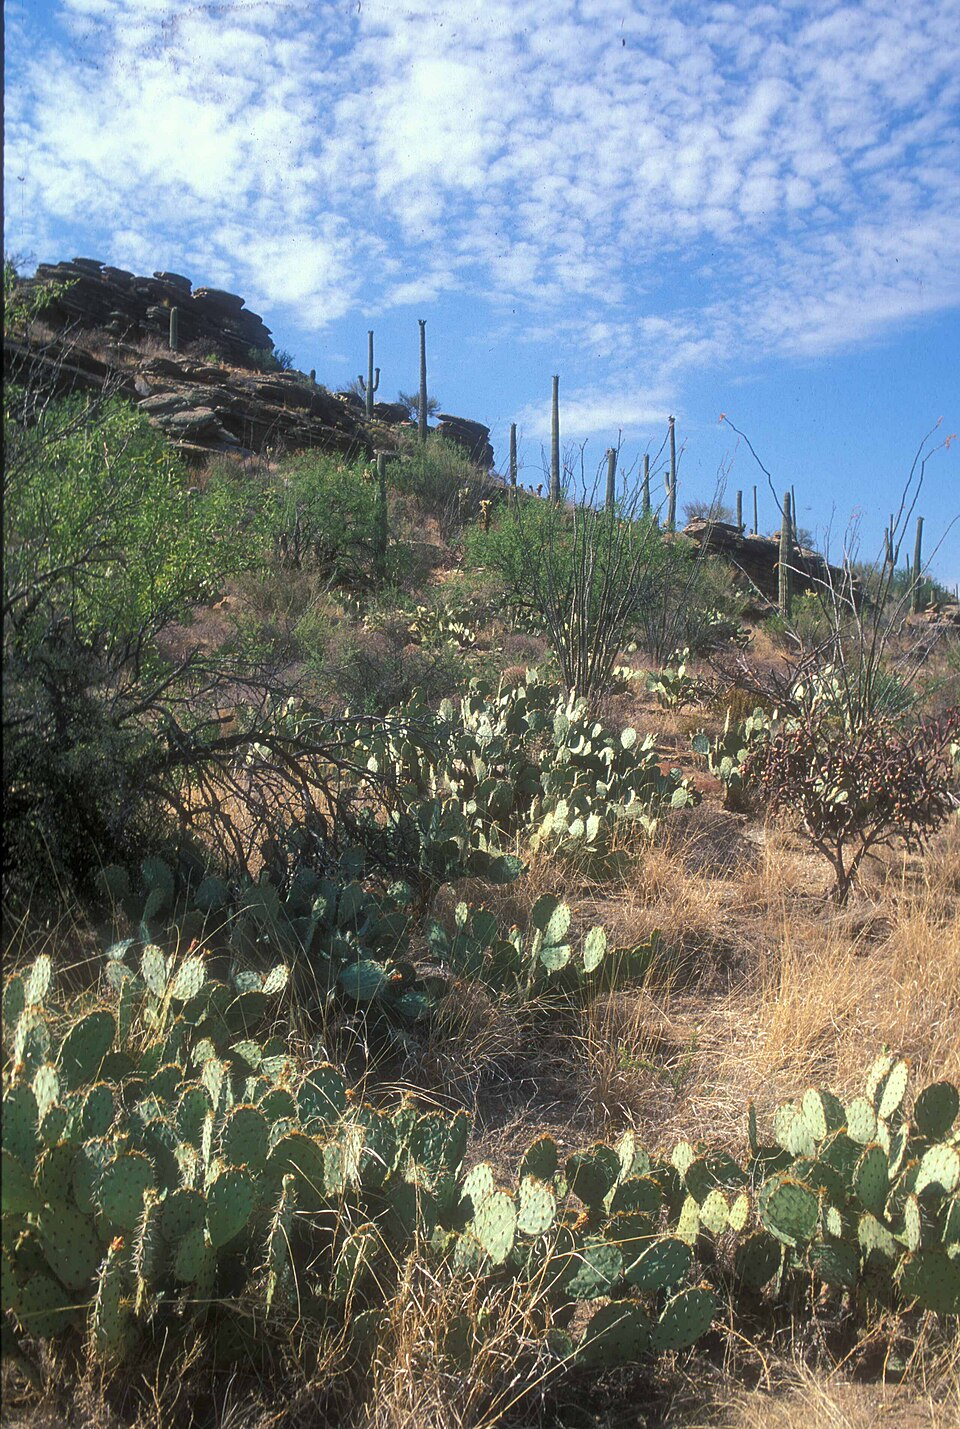
\includegraphics[height=3.6cm]{images/book1/g5-sonoran-desert.jpg}\quad
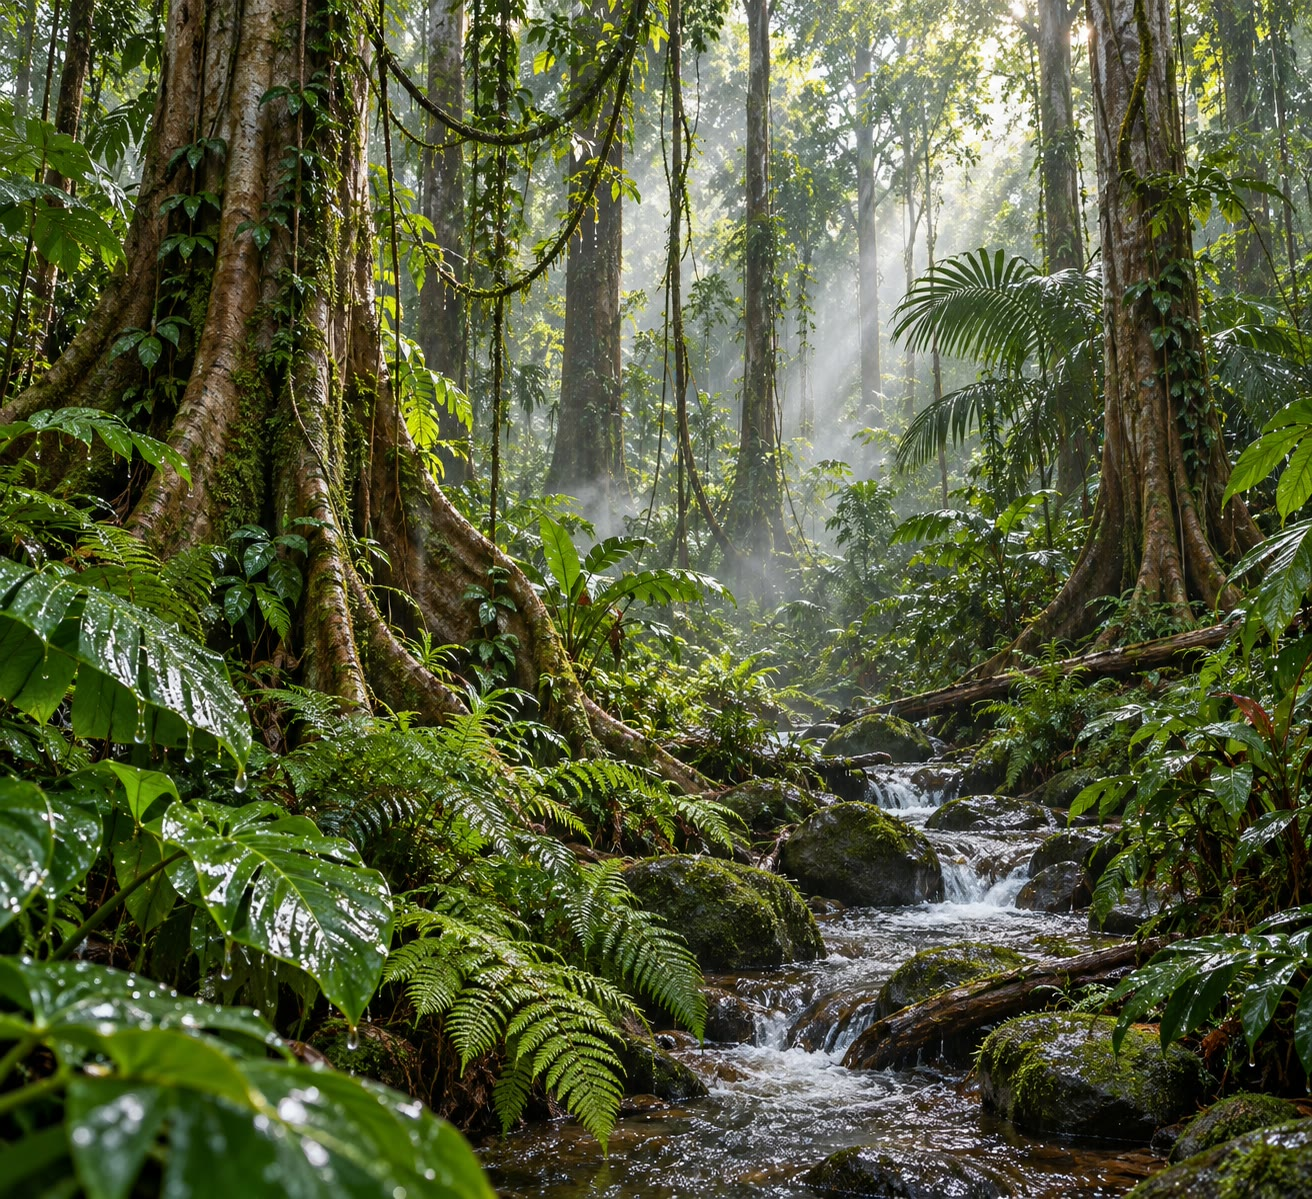
\includegraphics[height=3.6cm]{images/book1/ai/g5-rainforest.jpg}\quad
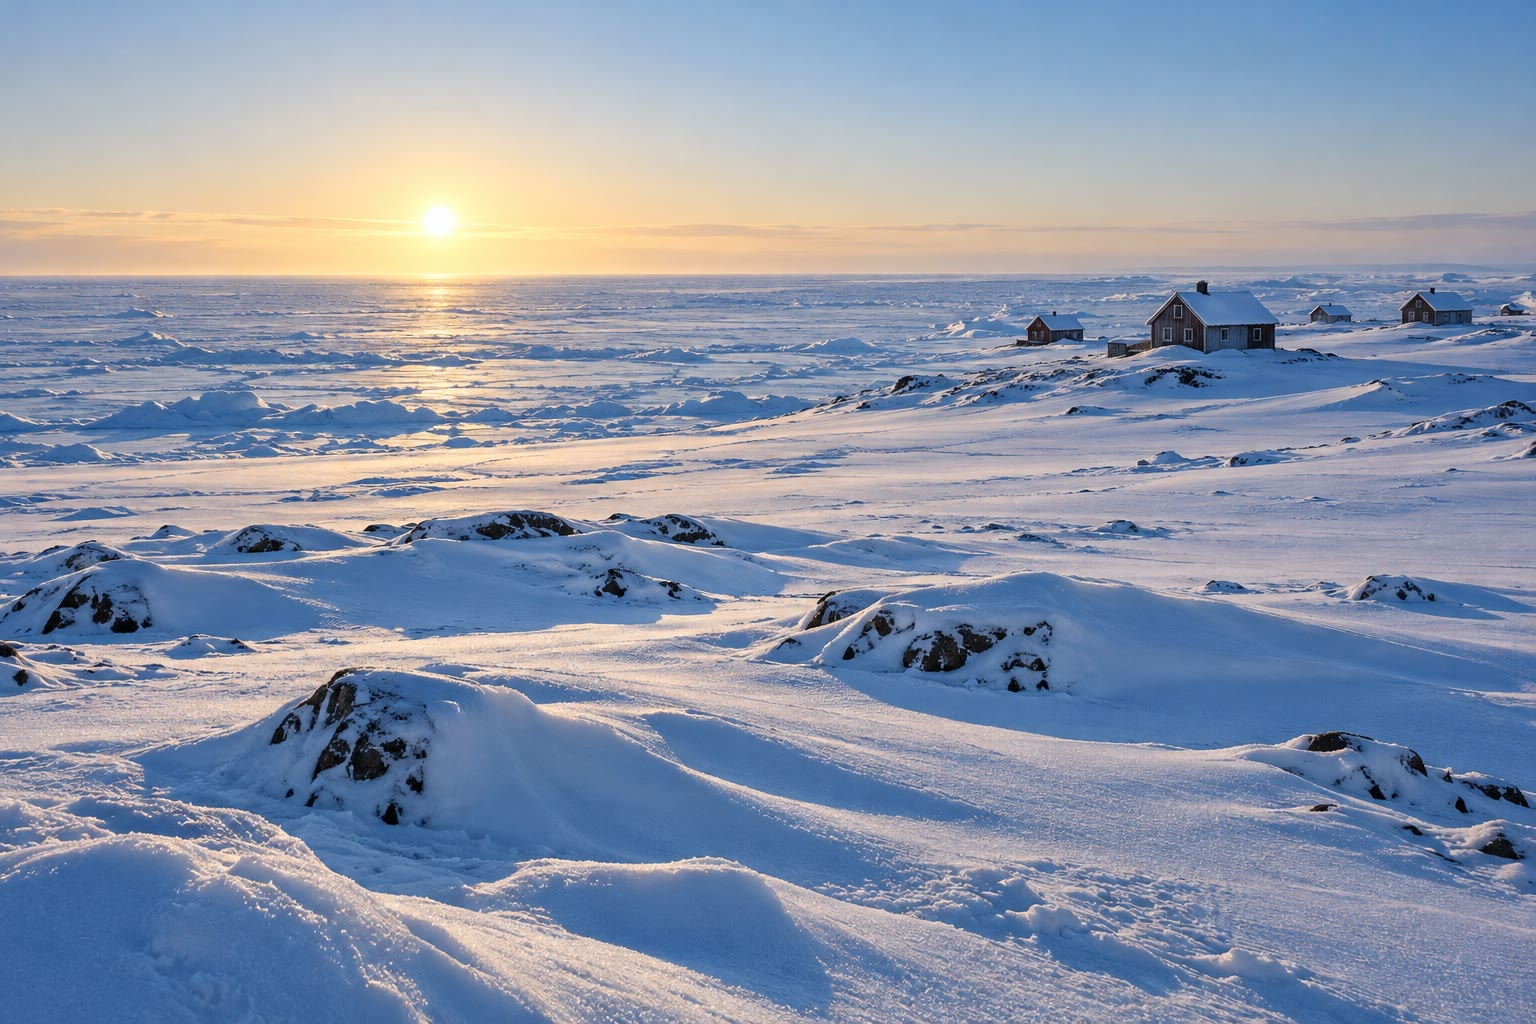
\includegraphics[height=3.6cm]{images/book1/ai/g5-polar-tundra.jpg}

{\small ثلاثة مناخات قصوى. إلى اليمين: \omterm{def:g5:weather-and-climate:desert}{صحراء} سونورا في أريزونا، \omterm{def:g5:weather-and-climate:desert}{صحراء}
فينيكس، بصبّاراتها الساغوارو الطويلة وصبّارات التين الشوكي، التي تخزن
الماء في سيقانها السميكة (الصورة: مصلحة المتنزهات الوطنية الأمريكية، متنزه
ساغوارو الوطني، ملك عام). في الوسط: داخل \omterm{def:g5:weather-and-climate:rainforest}{غابة مطيرة} بعد زخة \omterm{def:g4:clouds-rain-snow:precipitation}{مطر}.
إلى اليسار: \omterm{def:g1:landscapes-around-us:water}{ساحل} قطبي في الشتاء، مع \omterm{def:g2:water-on-earth:ocean}{بحر} متجمد وشمس منخفضة عند الظهر.}
% ledger: nps:sonoran-desert
\end{omfigure}

\paragraph{المناخ المعتدل.} سياتل في الوسط: منحناها يرتفع
في الصيف وينخفض في الشتاء، لكن ليس كثيرًا أبدًا؛ ومطرها وفير إلى حد ما،
وأكثره في الخريف والشتاء. هذا \omterm{def:g5:weather-and-climate:climate}{مناخ} معتدل: لا حر شديد،
ولا برد شديد.

\paragraph{المناخ القطبي.} في أوتكياغفيك، يبقى المنحنى الأحمر تحت
\babelsublr{0~$^\circ$C} ثمانية أشهر من السنة؛ وفي فبراير يكون المتوسط
24 درجة تحت الصفر. وحتى في يوليو، أدفأ الأشهر، لا يتجاوز نحو
5 درجات.
% ledger: data:b1-noaa-normals

\section{النطاقات الحارة والمعتدلة والباردة}

لماذا يكون الجو دافئًا قرب \omterm{def:g3:continents-and-oceans:equator}{خط الاستواء} وباردًا قرب \omterm{def:g3:continents-and-oceans:poles}{القطبين}؟ بسبب
الشمس. فقرب \omterm{def:g3:continents-and-oceans:equator}{خط الاستواء}، تقف شمس الظهر عالية في السماء طوال
السنة: فيسقط ضوؤها عموديًا تقريبًا ويسخّن الأرض بقوة.
أما قرب \omterm{def:g3:continents-and-oceans:poles}{القطبين}، فتبقى الشمس منخفضة دائمًا: فيصل ضوؤها مائلًا،
موزعًا على مساحة كبيرة، فلا يسخّن إلا قليلًا. وفي الشتاء هناك، قد لا تشرق
الشمس أبدًا.

زوجان من الخطوط حول \omterm{def:g3:continents-and-oceans:globe}{مجسم الكرة الأرضية} يقسمان الأرض إلى \omterm{def:g5:weather-and-climate:climate-zone}{نطاقات مناخية}.

\begin{definition}[المداران والدائرتان القطبيتان]\label{def:g5:weather-and-climate:tropics}
\emph{المداران}\index{مدار} خطان حول \omterm{def:g3:continents-and-oceans:globe}{مجسم الكرة الأرضية}، أحدهما شمال
\omterm{def:g3:continents-and-oceans:equator}{خط الاستواء} والآخر جنوبه، يحددان أبعد مكان عن \omterm{def:g3:continents-and-oceans:equator}{خط الاستواء} يمكن أن تكون فيه
شمس الظهر عمودية فوق الرأس تمامًا: مدار السرطان في الشمال،
ومدار الجدي في الجنوب. و\emph{الدائرتان
القطبيتان}\index{دائرة قطبية} خطان حول \omterm{def:g3:continents-and-oceans:globe}{مجسم الكرة الأرضية}، قرب
\omterm{def:g3:continents-and-oceans:poles}{القطبين}، لا تشرق الشمس وراءهما في منتصف الشتاء يومًا واحدًا على
الأقل، ولا تغرب في منتصف الصيف: الدائرة القطبية الشمالية
في الشمال، والدائرة القطبية الجنوبية في الجنوب.
\end{definition}

ميل محور الأرض هو الذي يحدد مواضع هذه الخطوط.

\begin{definition}[النطاقات المناخية]\label{def:g5:weather-and-climate:climate-zone}
تنقسم الأرض إلى ثلاثة أنواع من \emph{النطاقات المناخية}\index{نطاق مناخي}: \emph{النطاق الحار}، بين المدارين، حول \omterm{def:g3:continents-and-oceans:equator}{خط الاستواء}؛
و\emph{النطاقان المعتدلان}، بين \omterm{def:g5:weather-and-climate:tropics}{مدار} \omterm{def:g5:weather-and-climate:tropics}{ودائرة قطبية}، حيث
يختلف الصيف عن الشتاء؛ و\emph{النطاقان الباردان}، وراء
الدائرتين القطبيتين، حول \omterm{def:g3:continents-and-oceans:poles}{القطبين}.
\end{definition}

\begin{omfigure}
\begin{tikzpicture}
\begin{axis}[ommap, width=\linewidth, xtick=\empty, ytick=\empty, grid=none,
    axis background/.style={fill=white}, clip=true]
  \addplot[fill=orange!35, draw=none] table {figdata/out/grade-5-climate_zones-hot.dat};
  \addplot[fill=green!20, draw=none] table {figdata/out/grade-5-climate_zones-temperate.dat};
  \addplot[fill=cyan!20, draw=none] table {figdata/out/grade-5-climate_zones-cold.dat};
  \addplot[fill=black!25, fill opacity=0.8, draw=black!60, line width=0.2pt]
    table {figdata/out/shared-geo-land.dat};
  \addplot[black!70, dashed, line width=0.5pt] table {figdata/out/grade-5-climate_zones-lines.dat};
  \draw[black!70, line width=0.6pt] (axis cs:-180,0) -- (axis cs:180,0);
  \addplot[only marks, mark=*, mark size=1.8pt, red!80!black]
    table[x=lon, y=lat] {figdata/out/grade-5-climate_zones-stations.dat};
  \begin{scope}[every node/.style={font=\scriptsize, fill=white, fill opacity=0.75,
      text opacity=1, inner sep=1pt}]
    \node[anchor=west] at (axis cs:-107,33.4) {فينيكس};
    \node[anchor=east] at (axis cs:-158,19.7) {هيلو};
    \node[anchor=west] at (axis cs:-117,47.4) {سياتل};
    \node[anchor=west] at (axis cs:-151,73.5) {أوتكياغفيك};
  \end{scope}
  \begin{scope}[every node/.style={font=\scriptsize\bfseries, align=center,
      fill=white, fill opacity=0.7, text opacity=1, inner sep=1pt}]
    \node at (axis cs:-5,83) {النطاق البارد};
    \node at (axis cs:-40,40) {النطاق المعتدل};
    \node at (axis cs:-25,-8) {النطاق الحار};
    \node at (axis cs:95,-45) {النطاق المعتدل};
    \node at (axis cs:-60,-80) {النطاق البارد};
  \end{scope}
\end{axis}
\end{tikzpicture}

{\small \omterm{def:g5:weather-and-climate:climate-zone}{النطاقات المناخية}. من الأعلى إلى الأسفل، الخطوط المتقطعة هي
\omterm{def:g5:weather-and-climate:tropics}{الدائرة القطبية} الشمالية، \omterm{def:g5:weather-and-climate:tropics}{ومدار} السرطان، \omterm{def:g5:weather-and-climate:tropics}{ومدار} الجدي، \omterm{def:g5:weather-and-climate:tropics}{والدائرة القطبية}
الجنوبية؛ والخط المتصل هو \omterm{def:g3:continents-and-oceans:equator}{خط الاستواء}. والنقاط الحمراء هي المدن الأربع
في \omterm{def:g5:weather-and-climate:climate-chart}{المخططات المناخية} أعلاه.}
% ledger: earth:obliquity, data:b1-noaa-normals
\end{omfigure}

النطاقات تعطي صورة أولى تقريبية. وفي داخل كل نطاق، أشياء كثيرة أخرى
تغيّر \omterm{def:g5:weather-and-climate:climate}{المناخ}: بُعد المكان عن \omterm{def:g2:water-on-earth:ocean}{البحر}، وارتفاعه، والجهة التي تأتي منها
رياحه. وستتعرف إليها في الصفوف اللاحقة.

\begin{remark}[فينيكس والنطاقات]\label{rem:g5:weather-and-climate:phoenix}
على \omterm{def:g2:drawing-to-map:map}{خريطة} النطاقات، تقع فينيكس شمال \omterm{def:g5:weather-and-climate:tropics}{مدار} السرطان بقليل،
في النطاق المعتدل، ومع ذلك فهي \omterm{def:g5:weather-and-climate:desert}{صحراء} حارة. فالنطاقات صورة
أولى تقريبية: كثير من \omterm{def:g5:weather-and-climate:desert}{الصحاري} الحارة الكبرى يقع قرب المدارين،
على حافة النطاق الحار، وستعرف السبب في
\cref{ch:g8:winds-global-circulation}.
\end{remark}

\section{تمارين}

\begin{exercise}[$\star$]\label{exo:g5:weather-and-climate:1}
\omterm{def:g1:watching-the-weather:weather}{طقس} أم \omterm{def:g5:weather-and-climate:climate}{مناخ}؟
\begin{enumerate}
  \item[(أ)] إنها تثلج في أوتكياغفيك هذا الصباح.
  \item[(ب)] في فينيكس، الصيف حار جدًا وجاف.
  \item[(ج)] بعد ظهر أمس هبت ريح قوية في سياتل.
  \item[(د)] في هيلو، تمطر كثيرًا في كل شهر من أشهر السنة.
\end{enumerate}
\end{exercise}

\begin{exercise}[$\star$]\label{exo:g5:weather-and-climate:2}
ما \omterm{def:g5:weather-and-climate:climate}{مناخ} مكان ما؟ وعلى مدى كم سنة يأخذ علماء \omterm{def:g1:watching-the-weather:weather}{الطقس} متوسط
قياساتهم ليصفوه؟
\end{exercise}

\begin{exercise}[$\star$]\label{exo:g5:weather-and-climate:3}
على \omterm{def:g5:weather-and-climate:climate-chart}{المخطط المناخي} لسياتل، أي الأشهر أبردها؟ وأيها
أكثرها مطرًا؟ وهل تنزل درجة الحرارة يومًا تحت \babelsublr{0~$^\circ$C}؟
\end{exercise}

\begin{exercise}[$\star$]\label{exo:g5:weather-and-climate:4}
على \omterm{def:g5:weather-and-climate:climate-chart}{المخطط المناخي} لأوتكياغفيك، أي الأشهر أدفؤها؟ وهل يوجد
شهر أدفأ من \babelsublr{10~$^\circ$C}؟
\end{exercise}

\begin{exercise}[$\star$]\label{exo:g5:weather-and-climate:5}
في أي \omterm{def:g5:weather-and-climate:climate-zone}{نطاق مناخي} يقع كل مكان من هذه الأماكن: \omterm{def:g3:continents-and-oceans:equator}{خط الاستواء}؛ \omterm{def:g3:continents-and-oceans:poles}{القطب
الشمالي}؛ مكان في منتصف المسافة بين \omterm{def:g3:continents-and-oceans:equator}{خط الاستواء} \omterm{def:g3:continents-and-oceans:poles}{والقطب الجنوبي}؟
\end{exercise}

\begin{exercise}[$\star$]\label{exo:g5:weather-and-climate:6}
استعن \omterm{def:g2:drawing-to-map:map}{بخريطة} النطاقات. في أي \omterm{def:g5:weather-and-climate:climate-zone}{نطاق مناخي} تقع كل مدينة من المدن الأربع:
فينيكس، هيلو، سياتل، أوتكياغفيك؟
\end{exercise}

\begin{exercise}[$\star\star$]\label{exo:g5:weather-and-climate:7}
هذا متوسط \omterm{def:g4:clouds-rain-snow:precipitation}{المطر} في كل شهر في سياتل، بالمليمترات، مقرّبًا
إلى أعداد صحيحة (الأشهر مرقّمة من 1، يناير، إلى 12، ديسمبر):
\begin{center}
\begin{tabular}{|*{12}{c|}}
\hline
1 & 2 & 3 & 4 & 5 & 6 & 7 & 8 & 9 & 10 & 11 & 12\\
\hline
147 & 96 & 106 & 81 & 48 & 37 & 15 & 25 & 41 & 99 & 160 & 145\\
\hline
\end{tabular}
\end{center}
كم من \omterm{def:g4:clouds-rain-snow:precipitation}{المطر} يسقط في سياتل في السنة كلها؟ وكم يسقط في
الأشهر الثلاثة ديسمبر ويناير وفبراير؟
% ledger: data:b1-noaa-normals
\end{exercise}

\begin{exercise}[$\star\star$]\label{exo:g5:weather-and-climate:8}
في فينيكس، متوسط درجة الحرارة \babelsublr{14~$^\circ$C} في يناير
و\babelsublr{35~$^\circ$C} في يوليو. وفي هيلو، \babelsublr{22~$^\circ$C} في يناير
و\babelsublr{25~$^\circ$C} في يوليو. احسب الفرق بين يوليو ويناير في
كل مدينة. أين تغيّر الفصول درجة الحرارة أكثر؟
% ledger: data:b1-noaa-normals
\end{exercise}

\begin{exercise}[$\star\star$]\label{exo:g5:weather-and-climate:9}
هذه متوسطات مدينة خيالية (الأشهر مرقّمة من 1، يناير، إلى 12، ديسمبر).
\begin{center}
\begin{tabular}{|l|*{12}{c|}}
\hline
الشهر & 1 & 2 & 3 & 4 & 5 & 6 & 7 & 8 & 9 & 10 & 11 & 12\\
\hline
درجة الحرارة \babelsublr{($^\circ$C)} & 27 & 27 & 28 & 28 & 28 & 27 & 27 & 27 & 27 & 27 & 27 & 27\\
\hline
\omterm{def:g4:clouds-rain-snow:precipitation}{المطر} (mm) & 250 & 230 & 280 & 290 & 260 & 180 & 170 & 160 & 190 & 230 & 250 & 260\\
\hline
\end{tabular}
\end{center}
أهو \omterm{def:g5:weather-and-climate:climate}{مناخ} \omterm{def:g5:weather-and-climate:desert}{صحراء}، أم \omterm{def:g5:weather-and-climate:rainforest}{غابة مطيرة}، أم \omterm{def:g5:weather-and-climate:climate}{مناخ} معتدل، أم \omterm{def:g5:weather-and-climate:climate}{مناخ} قطبي؟ أعطِ
سببين. وفي أي نطاق يُرجّح أن تقع المدينة؟
\end{exercise}

\begin{exercise}[$\star\star$]\label{exo:g5:weather-and-climate:10}
عد إلى البطاقتين البريديتين في بداية الفصل، المرسلتين في الأسبوع نفسه
من يناير. أعطِ تفسيرين مختلفين لكيف يمكن لأطفال أن يلعبوا
على شاطئ مشمس في مكان، بينما يبني آخرون رجل \omterm{def:g4:clouds-rain-snow:precipitation}{ثلج} في مكان آخر.
\end{exercise}

\begin{exercise}[$\star\star\star$]\label{exo:g5:weather-and-climate:11}
تقول نور: «فينيكس وسياتل كلتاهما في النطاق المعتدل، فلا بد أن
يكون لهما \omterm{def:g5:weather-and-climate:climate}{المناخ} نفسه.» استعن \omterm{def:g5:weather-and-climate:climate-chart}{بالمخططات المناخية} لتبين أنها
مخطئة: قارن درجات حرارتهما ومطرهما. ثم قل ما تخبرنا به \omterm{def:g5:weather-and-climate:climate-zone}{النطاقات
المناخية}، وما لا تخبرنا به.
\end{exercise}
